\documentclass[12pt]{article}

\usepackage{sbc-template}
\usepackage{graphicx,url}
\usepackage[utf8]{inputenc}
\usepackage[brazil]{babel}
\usepackage{amsmath}

% Gerado automaticamente por src/fill_paper.py - nao editar a mao.
\newcommand{\AUCImbBal}{0{,}688}
\newcommand{\AUCImbNone}{0{,}699}
\newcommand{\AUCImbSmote}{0{,}681}
\newcommand{\AblClaheDelta}{+0{,}007}
\newcommand{\AblDefaultAUC}{0{,}710}
\newcommand{\AblMaskDelta}{+0{,}014}
\newcommand{\AblRawAUC}{0{,}692}
\newcommand{\AccMaskFb}{0{,}821}
\newcommand{\AccMaskOk}{0{,}621}
\newcommand{\AccModCR}{0{,}665}
\newcommand{\AccModDX}{0{,}614}
\newcommand{\AllBestAUC}{0{,}710}
\newcommand{\AtyToTyp}{68{,}5\%}
\newcommand{\BalAccBal}{0{,}426}
\newcommand{\BalAccNone}{0{,}392}
\newcommand{\BalAccSmote}{0{,}416}
\newcommand{\BestConfig}{Todas + SVM-RBF}
\newcommand{\BestFamily}{HOG}
\newcommand{\BestFamilyAUC}{0{,}702}
\newcommand{\BestModelAvg}{SVM-RBF}
\newcommand{\BinAUCModCR}{0{,}885}
\newcommand{\BinAUCModDX}{0{,}835}
\newcommand{\DevAUC}{0{,}710 $\pm$ 0{,}014}
\newcommand{\DevBalAcc}{0{,}395}
\newcommand{\IndToTyp}{64{,}2\%}
\newcommand{\MaskFallback}{9{,}2\%}
\newcommand{\NDev}{4.780}
\newcommand{\NImages}{6.334}
\newcommand{\NPatients}{3.261}
\newcommand{\NStudies}{6.054}
\newcommand{\NTest}{1.274}
\newcommand{\PctAty}{7{,}8\%}
\newcommand{\PctInd}{17{,}3\%}
\newcommand{\PctNeg}{27{,}7\%}
\newcommand{\PctTyp}{47{,}2\%}
\newcommand{\PrevPneuMaskFb}{97{,}4\%}
\newcommand{\PrevPneuMaskOk}{69{,}7\%}
\newcommand{\SensAty}{1{,}1\%}
\newcommand{\SensAtyBal}{0{,}333}
\newcommand{\SensAtyNone}{0{,}028}
\newcommand{\SensAtySmote}{0{,}300}
\newcommand{\SensInd}{2{,}0\%}
\newcommand{\SensNeg}{74{,}3\%}
\newcommand{\SensTyp}{87{,}2\%}
\newcommand{\TestAP}{0{,}463}
\newcommand{\TestAPDummy}{0{,}250}
\newcommand{\TestAUC}{0{,}729}
\newcommand{\TestAUCEn}{0.729}
\newcommand{\TestBalAcc}{0{,}412}
\newcommand{\TestBinAUC}{0{,}861}
\newcommand{\TestFone}{0{,}370}
\newcommand{\TopFamily}{HOG}
\newcommand{\TopFamilyDrop}{0{,}195}
\newcommand{\TopFeature}{hog\_1073}
\newcommand{\WorstModelAvg}{Random Forest}


\sloppy

\title{Baseline Cl\'assico para Radiografias de T\'orax\\no Desafio SIIM-FISABIO-RSNA COVID-19}

\author{Felipe Freires da Costa\inst{1}, Eduardo Nobre Nogueira de Oliveira\inst{1},\\
Pedro Paulo Alves dos Santos Nunes\inst{1}}

\address{Curso de Sistemas de Informa\c{c}\~ao -- NOME DA INSTITUI\c{C}\~AO\\
CIDADE -- UF -- Brasil
\email{\{felipe,eduardo,pedro\}@DOMINIO.edu.br}
}

\begin{document}

\maketitle

\begin{abstract}
We build a non-deep-learning baseline for four-class study-level classification of chest
radiographs in the 2021 SIIM-FISABIO-RSNA COVID-19 challenge: five hand-crafted descriptor
families from a classical lung mask, four classifiers and patient-grouped nested
cross-validation. On a frozen hold-out, the selected model reaches a macro AUC-ROC of
\TestAUCEn{} (trivial: 0.500); most errors are indeterminate and atypical studies predicted
as typical.
\end{abstract}

\begin{resumo}
Constru\'{\i}mos um baseline sem aprendizado profundo para classificar, por estudo,
radiografias de t\'orax em quatro classes no desafio SIIM-FISABIO-RSNA COVID-19 (2021): cinco
fam\'{\i}lias de descritores manuais de uma m\'ascara pulmonar cl\'assica, quatro classificadores
e valida\c{c}\~ao cruzada aninhada agrupada por paciente. No teste congelado, o modelo
selecionado atinge AUC-ROC macro de \TestAUC{} (trivial: 0,500); a maior parte dos erros s\~ao
estudos indeterminados e at\'{\i}picos preditos como t\'{\i}picos.
\end{resumo}

\section{Introdu\c{c}\~ao}

Na COVID-19, a radiografia de t\'orax (RX) mostra opacidades inespec\'{\i}ficas, em geral
bilaterais, perif\'ericas e basais \cite{wong2020frequency}; o laudo padronizado as classifica
em apar\^encia t\'{\i}pica, indeterminada, at\'{\i}pica ou negativa \cite{litmanovich2020review}. O desafio SIIM-FISABIO-RSNA de 2021 adotou essas categorias em
um conjunto multic\^entrico anotado por radiologistas \cite{lakhani2023siim}; formulamos a
tarefa como classifica\c{c}\~ao em quatro classes \emph{por estudo}. Como modelos profundos em RX
tendem a aprender atalhos \cite{degrave2021shortcuts}, \'e preciso um piso interpret\'avel e
medido com rigor. Contribu\'{\i}mos com:
\begin{itemize}
\item pipeline reprodut\'{\i}vel de leitura DICOM, m\'ascara pulmonar e cinco fam\'{\i}lias de
descritores, inclusive zonais;
\item grade descritor $\times$ classificador em CV aninhada por paciente, com baseline
trivial, teste congelado e abla\c{c}\~oes;
\item an\'alise de erro por classe, por modalidade (CR/DX) e por falha da m\'ascara.
\end{itemize}

\section{Trabalhos Relacionados}

M\'ascaras pulmonares com histogramas, bordas, LBP e HOG em SVM j\'a detectavam achados
difusos na triagem de tuberculose \cite{jaeger2014tb}, e descritores de textura foram
aplicados \`a COVID-19 em RX port\'ateis \cite{hussain2020texture}. Muitos desses estudos,
por\'em, usaram fontes distintas por classe e parti\c{c}\~ao por imagem, o que superestima o
desempenho \cite{roberts2021pitfalls} e favorece atalhos \cite{degrave2021shortcuts}. Usamos
rotulagem padronizada, sem classes ligadas a fontes distintas
\cite{lakhani2023siim}, e particionamos por paciente com CV aninhada \cite{varma2006bias}.

\section{Metodologia}

\textbf{Dados.} C\'odigo e parti\c{c}\~ao congelada (semente 42): \url{https://github.com/FelipeFreires-Costa/COVID-19-AI-Detection-AP1}. Usamos todo o treino do desafio (\NStudies{} estudos, \NImages{} imagens,
\NPatients{} pacientes), pois os r\'otulos do teste oficial n\~ao s\~ao p\'ublicos: T\'{\i}pico
\PctTyp{}, Negativo \PctNeg{}, Indeterminado \PctInd{} e At\'{\i}pico \PctAty{}. Com
\texttt{StratifiedGroupKFold} por \texttt{PatientID}, separamos dev (\NDev{} estudos,
5 dobras) e teste (\NTest{} estudos), sem paciente em comum.

\textbf{Pr\'e-processamento.} Aplicamos \emph{Modality LUT} (\emph{RescaleSlope/Intercept}) e
\emph{VOI LUT}, invertemos imagens MONOCHROME1, normalizamos pelos percentis 0,5--99,5,
redimensionamos para $512\times512$ e aplicamos CLAHE \cite{zuiderveld1994clahe}. A m\'ascara
pulmonar segue o limiar de Otsu \cite{otsu1979} com regras morfol\'ogicas, como em \cite{jaeger2014tb}: abertura, os dois maiores componentes internos e fecho
convexo; quando falha, usamos uma ROI fixa (\MaskFallback{} das imagens). Ela \'e dividida
em seis zonas (lado $\times$ ter\c{c}o vertical).

\textbf{Descritores}, dentro da m\'ascara: (1) \emph{intensidade zonal} (momentos, percentis,
histograma, estat\'{\i}sticas por zona, assimetria lateral e gradiente inferior-superior), que
codifica a distribui\c{c}\~ao t\'{\i}pica \cite{wong2020frequency}; (2) \emph{GLCM/Haralick}
\cite{haralick1973} (7 propriedades, 3 dist\^ancias, 4 \^angulos), para a heterogeneidade do
vidro fosco; (3) \emph{LBP} uniforme invariante \`a rota\c{c}\~ao em 3 escalas
\cite{ojala2002lbp}, pela invari\^ancia a mudan\c{c}as monot\^onicas de brilho; (4) \emph{Gabor}
\cite{jain1991gabor} (4 escalas, 4 orienta\c{c}\~oes); e (5) \emph{HOG} \cite{dalal2005hog} no
recorte pulmonar. Estudos com v\'arias imagens usam a m\'edia.

\textbf{Modelos e protocolo.} Comparamos o baseline trivial (probabilidades a priori) com
regress\~ao log\'{\i}stica, SVM-RBF, Random Forest e LightGBM \cite{ke2017lightgbm}, com pesos de
classe balanceados, via scikit-learn \cite{pedregosa2011sklearn}. Imputa\c{c}\~ao, padroniza\c{c}\~ao
e PCA ficam no \emph{pipeline}, ajustados s\'o no treino de cada dobra. Os hiperpar\^ametros
s\~ao escolhidos em 3 dobras internas agrupadas dentro de cada uma das 5 externas
\cite{varma2006bias}; a melhor no dev \'e reajustada e avaliada uma \'unica vez no teste. Reportamos AUC-ROC e AUC-PR macro (esta mais informativa sob desbalanceamento
\cite{saito2015pr}), acur\'acia balanceada, sensibilidade por classe e AUC bin\'aria pneumonia
vs.\ negativo.

\section{Resultados e Discuss\~ao}

% PLACEHOLDER - substituir pelo arquivo gerado em results/tables/table_main.tex
\begin{table}[ht]
\centering
\caption{AUC-ROC macro (um-contra-todos) na valida\c{c}\~ao cruzada aninhada (5 dobras externas agrupadas por paciente), m\'edia $\pm$ desvio-padr\~ao.}
\label{tab:main}
\small
\begin{tabular}{lcccc}
\hline
Descritor & Reg. Log\'{\i}stica & SVM-RBF & Random Forest & LightGBM \\
\hline
Intensidade (zonal) & XX & XX & XX & XX \\
GLCM/Haralick & XX & XX & XX & XX \\
LBP & XX & XX & XX & XX \\
Gabor & XX & XX & XX & XX \\
HOG & XX & XX & XX & XX \\
Todas & XX & XX & XX & XX \\
\hline
Baseline trivial (majorit\'ario) & \multicolumn{4}{c}{0.500 $\pm$ 0.000} \\
\hline
\end{tabular}
\end{table}


A melhor fam\'{\i}lia isolada foi \BestFamily{} (AUC \BestFamilyAUC{}); a concatena\c{c}\~ao de
todas chegou a \AllBestAUC{} (Tabela~\ref{tab:main}) e, em m\'edia, \BestModelAvg{} foi o melhor
classificador. A selecionada, \BestConfig{}, teve AUC \DevAUC{} na CV e, no teste, AUC
\TestAUC{}, AUC-PR \TestAP{} (trivial: \TestAPDummy{}), acur\'acia balanceada \TestBalAcc{}
(trivial: 0,250) e AUC bin\'aria \TestBinAUC{}.

\begin{figure}[ht]
\centering
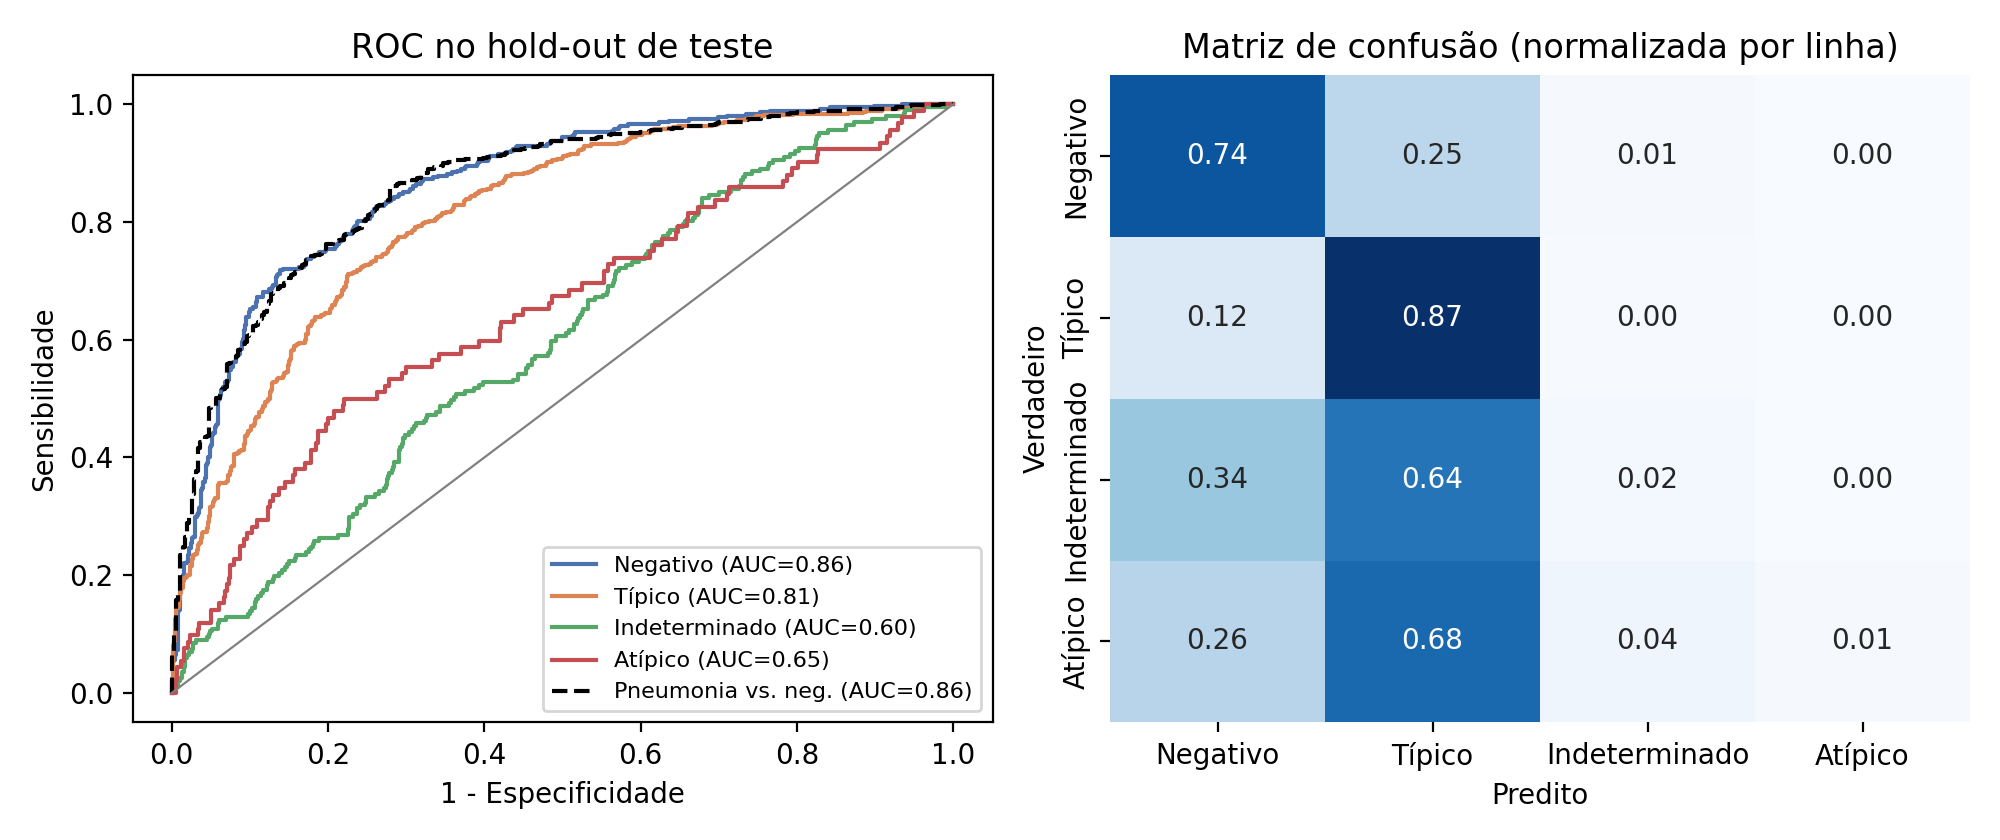
\includegraphics[width=0.56\textwidth]{figures/fig_roc_cm.png}
\caption{ROC por classe e matriz de confus\~ao normalizada no teste.}
\label{fig:roccm}
\end{figure}

\textbf{Abla\c{c}\~oes.} A AUC foi \AblRawAUC{} sem CLAHE e sem m\'ascara e \AblDefaultAUC{} no
pipeline completo: a m\'ascara contribuiu com \AblMaskDelta{} e o CLAHE com \AblClaheDelta{}.
Com regress\~ao log\'{\i}stica, a sensibilidade da classe At\'{\i}pica foi \SensAtyNone{} sem
tratamento, \SensAtyBal{} com pesos de classe e \SensAtySmote{} com SMOTE
\cite{chawla2002smote}, enquanto a AUC pouco variou (\AUCImbNone{}, \AUCImbBal{},
\AUCImbSmote{}): o tratamento desloca sobretudo o limiar.

\textbf{An\'alise de erro.} No teste, \IndToTyp{} dos Indeterminados e \AtyToTyp{} dos
At\'{\i}picos foram preditos como T\'{\i}picos (Figura~\ref{fig:roccm}): as categorias diferem mais
pela distribui\c{c}\~ao das opacidades que pela textura \cite{litmanovich2020review}, o que
descritores agregados captam s\'o em parte. A acur\'acia maior no fallback (\AccMaskFb{}
contra \AccMaskOk{}) \'e enganosa: \PrevPneuMaskFb{} desses estudos t\^em pneumonia (contra
\PrevPneuMaskOk{} com m\'ascara v\'alida), pois opacidades densas quebram o limiar de Otsu e
favorecem a classe T\'{\i}pico. A acur\'acia foi \AccModCR{} em CR e \AccModDX{} em DX (AUC
bin\'aria \BinAUCModCR{} e \BinAUCModDX{}); na permuta\c{c}\~ao, \TopFamily{} foi a fam\'{\i}lia
mais informativa.

\section{Conclus\~ao}

O baseline cl\'assico fixa o piso do projeto em AUC-ROC macro de \TestAUC{} e acur\'acia
balanceada de \TestBalAcc{}: h\'a sinal para detectar pneumonia, mas pouco para separar as
apar\^encias at\'{\i}pica e indeterminada, de defini\c{c}\~ao espacial. Limita\c{c}\~oes: m\'ascara
heur\'{\i}stica, agrega\c{c}\~ao por m\'edia e falta de harmoniza\c{c}\~ao entre equipamentos. Pr\'oximos
passos: descritores regionais guiados pelas caixas de opacidade e compara\c{c}\~ao com redes
profundas na mesma parti\c{c}\~ao.

\bibliographystyle{sbc}
\bibliography{refs}

\noindent\footnotesize\textbf{Uso de IA generativa:} apoio em d\'uvidas de c\'odigo, revis\~ao,
tradu\c{c}\~ao e formula\c{c}\~ao de trechos; conte\'udo e refer\^encias revisados pelo grupo.\normalsize

\end{document}
